\section{Conceptual Framework} 

\subsection{Eye Tracking}

Eye Tracking refers to "the use of proper techniques and tools for the identification of a subject's gaze direction; in other words, eye tracking allows detecting and recording what users watch, typically, but not necessarily, on a screen" \citep{cantoni2014eye}. This technique can be measured and applied in different disciplines, which will be explained in the following sections.

\cite{dondi2023gaze} point out that there are mainly two different kinds of Eye Trackers:
\begin{enumerate}
    \item \textit{Remote}, the selected type for the project, which are non-intrusive devices positioned at the bottom of the display.
    \item \textit{Wearable}, that are installed in a pair of glasses, for instance, and are able to track outside of digital environments.
\end{enumerate}

\subsubsection{Gaze}

Gaze is usually associated with a fixed or steady look, however in this field it is used to describe the approximate point on screen where the subject is fixating their eyes. \cite{cantoni2014eye} have explained that to obtain this information in Eye Trackers, gaze direction is obtained during an initial calibration phase, which determines the correspondences between the points observed by the subject on the screen, and the positions of the cornea. 

\subsubsection{Accuracy and Precision}

These two concepts have various applications, like in data science for example, but can be used in this context to understand how the Eye Tracker is performing. Following the manufacturer definitions, accuracy refers to the discrepancy between the true gaze position and the location recorded by the eye tracker, reflecting the systematic error or spatial accuracy of the data. On the other hand, precision indicates the consistency of the eye tracker in capturing the same gaze point across successive samples. It is quantified using the Root Mean Square (RMS) of the recorded points to assess the variation in the data. \citep{accuracy-precision-tobii}

\begin{figure}[ht]
    \centering
    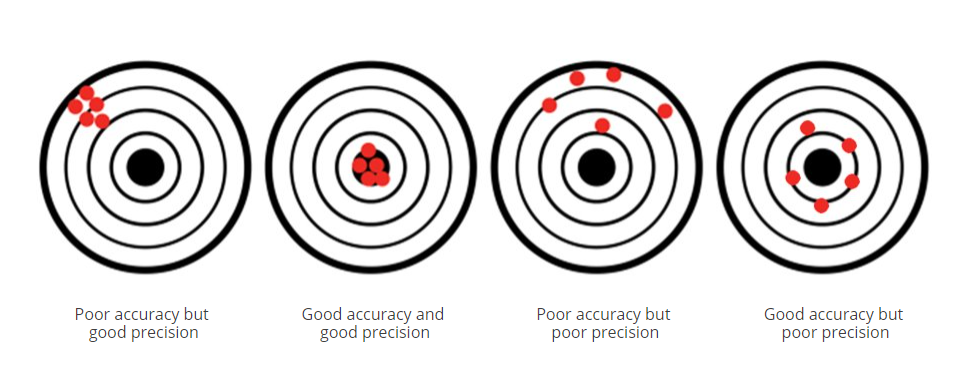
\includegraphics[width=0.4\textwidth]{images/accuracy-precision.jpeg}
    \caption{Accuracy and Precision. Source: \cite{accuracy-precision-tobii}}
    \label{fig:accuracy-precision-tobii}
\end{figure}

\subsubsection{Applications}

\begin{itemize}
    \item Usability testing
    
    In this field, eye tracking allows for the analysis of the behavior of the user. This is a process that occurs after they have used the product, which means it does not take an active role in the interaction per se. \citep{jacob2003commentary}

    \item Psychology experiments
    
    Many different psychology experiments can be done using eye tracking, for instance, the cognitive load students using a Learning Management System (LMS) has been analyzed using eye tracking, and how it had an effect on their learning outcomes. \citep{saiz2024using}

    \item Input method
    
    As \cite{jacob2003commentary} point out, the application of eye trackers in HCI (Human-Computer Interaction) has long been studied and researched. The approach of using eye tracking as an input method is yet to be applied massively in a commercial environment.

    \item Artificial Intelligence
    
    In the rising field of Generative Artificial Intelligence, \cite{taieb2024mining} used eye tracking to perform text summarization, mining data from attention metrics, which outperforms regular text summarization. 

\end{itemize}


\subsection{Natural Language Processing}

Natural Language Processing (NLP) is a field of artificial intelligence that focuses on the interaction between computers and humans through natural language. The goal of NLP is to enable computers to understand, interpret, and generate human language in a way that is both meaningful and useful. As \cite{book:3382520} describes it, "[Natural Language Processing] addresses the various ways in computers can deal with natural—that is human—language"

% TODO research and cite

\subsubsection{Applications}

\begin{itemize}
    \item Search engines
    \item Assistive technologies
    \item transcriptions
    \item Smart voice assistants
\end{itemize}


\subsection{Record And Replay Testing}

% TODO research and cites

\subsubsection{Gherkin Syntax}

All of the testing developed was possible thanks to the Kraken module developed by \cite{ravelo2023kraken}. These tests are made using the Gherkin syntax and WebdriverIO, which enables controlling the browser for automated testing scenarios.



